\section{Motivating Example}
\label{sec:example}

Consider the following SQL question picked up from a classic
database textbook~\cite{cowbook}: \textit{given a \CodeIn{student} table (Figure~\ref{tbl:student})
and an \CodeIn{enrolled} table (Figure~\ref{tbl:enrolled}), find out the name and max score of the
students whose level is senior and enrolled in more than 3 courses}.


\begin{figure*}[t]
  \centering
  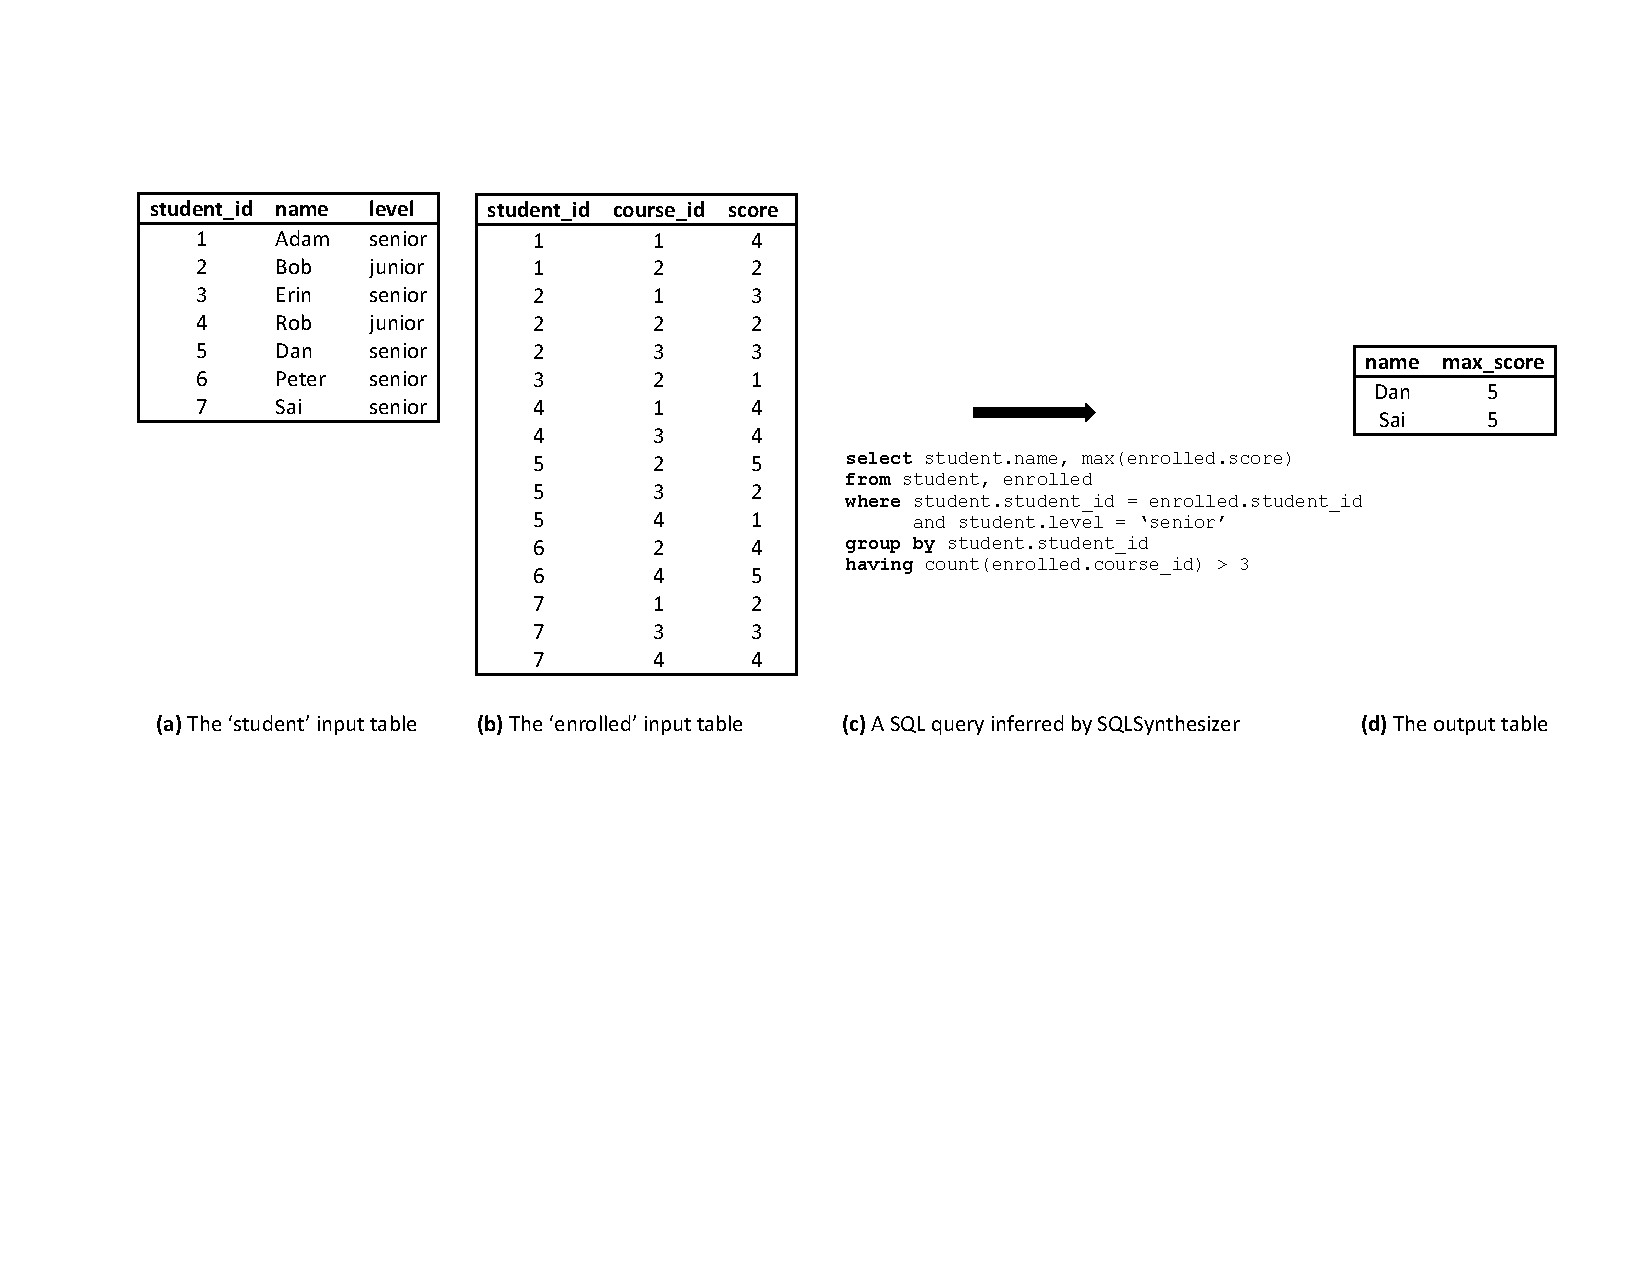
\includegraphics[scale=0.70]{motivating}
  \vspace*{-1.0ex}\caption {{\label{fig:motivating}
  Example input-output tables and the SQL query sythensized by
  \ourtool. In this example, users provide \ourtool with
  two input tables (shown in (a) and (b)) and an output table (shown in (d));
  \ourtool automatically infers a SQL query (shown in (c)) that
  transforms the two input tables into the output table.
}}
\end{figure*}


The question's description is quite simple.
For a novice user, although they have a clear
intention of what the query should do, the answer (Figure~\ref{fig:expected_sql}) may
not be that straightforward. 

Despite the possible difficult in writing a correct SQL query,
a user could still easily draw
two input tables (Figure~\ref{tbl:student} and Figure~\ref{tbl:enrolled})
and one output table (Figure~\ref{tbl:output}) that fulfill the
SQL question.

In the \CodeIn{student} table, column {\CodeIn{Student\_key}} with
\CodeIn{String} type serves as the primary key. 
%Columns {\CodeIn{Student\_name}} and {\CodeIn{Level}} are \textsf{String}-type.
In the \CodeIn{enrolled} table, both columns {\CodeIn{Student\_key}} and
{\CodeIn{Course\_key}} are two foreign keys, and column {\CodeIn{Score}}
with \CodeIn{Integer} type keeps students' scores on their enrolled courses.

In the output table, the first column  {\CodeIn{Student\_name}}
comes from table \textit{student}, and the second column {\CodeIn{Max\_score}}
is a aggregation attribute.% summarizing the with type of \CodeIn{Integer}.

Having the input and output examples, our technique successfully synthesizes
the desirable SQL query as shown in Figure~\ref{fig:expected_sql}.
